%%%%%%%%%%%%%%%
%
% $Autor:Abishek Senthilkumar $
% $Datum: 2022-06-16 06:54:43Z $
% $Pfad: WuSt/Skript/Produktspezifikation/powerpoint/NaiveBayesWithPython.tex $
% $Version: 4973 $
%
%
%%%%%%%%%%%%%%%




\Mysection{Introduction}


\begin{frame}{What is Naïve Bayes classifier}
	
	\begin{itemize}
	\item Naïve Bayes algorithm is a supervised learning algorithm, which is based on Bayes theorem and used for solving classification problems. 
	\item It is mainly used in text classification that includes a high- dimensional training dataset.
	\item Naïve Bayes Classifier is one of the simple and most effective Classification algorithms which helps in building the fast machine learning models that can make quick predictions.
	\item It is a probabilistic classifier, which means it predicts on the basis of the probability of an object.
	\end{itemize}

\end{frame}

\begin{frame}{Why is it called Naïve Bayes?}
	\textbf{Naïve}: Assumes \textbf{feature independence}; each feature independently contributes to classification
	
		\begin{figure}
		\centering
		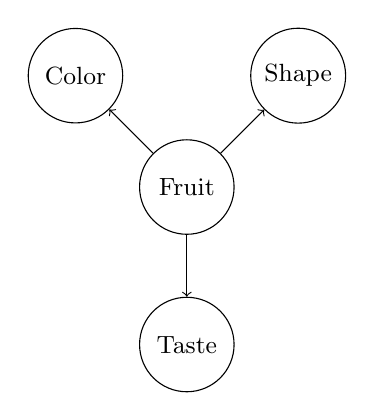
\begin{tikzpicture}[
			node distance=2.0cm,
			every node/.style={draw, circle, minimum size=1.2cm, text centered, font=\small}
			]
			% Nodes
			\node (class) {Fruit};
			\node[above left of=class] (color) {Color};
			\node[above right of=class] (shape) {Shape};
			\node[below of=class] (taste) {Taste};
			
			% Arrows representing independence
			\draw[->] (class) -- (color);
			\draw[->] (class) -- (shape);
			\draw[->] (class) -- (taste);
		\end{tikzpicture}
		\caption{Naïve Bayes Classifier Example}
		\label{fig:Naïve Bayes Classifier Example}
	\end{figure}
\end{frame}

\begin{frame}{Bayes Theorem}
	
	\textbf{Bayes' Theorem:} Also known as \textbf{Bayes' Rule} or \textbf{Bayes' Law}, it is used to determine the probability of a hypothesis based on prior knowledge and conditional probability.
	
	The formula for Bayes' theorem is given by:
	\[
	P(A|B) = \frac{P(B|A) \cdot P(A)}{P(B)}
	\]
	\textbf{Where:}
\begin{itemize}
	\item \( P(A|B) \): \textbf{Posterior Probability} - The probability of the hypothesis \( A \) given the observed event \( B \).
	\item \( P(B|A) \): \textbf{Likelihood Probability} - The probability of the evidence \( B \) given that hypothesis \( A \) is true.
	\item \( P(A) \): \textbf{Prior Probability} - The initial probability of the hypothesis \( A \) before observing any evidence.
	\item \( P(B) \): \textbf{Marginal Probability} - The probability of observing the evidence \( B \).
\end{itemize}
\end{frame}
\begin{frame}{Naïve Bayes Classification Process}
\begin{figure}
	\centering
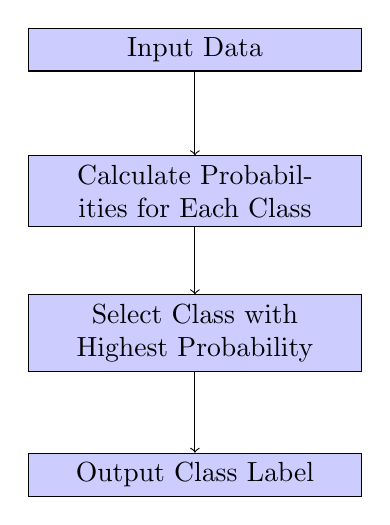
\begin{tikzpicture}[node distance=1.8cm, every node/.style={rectangle, draw, fill=blue!20, text width=4cm, align=center}]
	\node (input) {Input Data};
	\node (prob) [below of=input] {Calculate Probabilities for Each Class};
	\node (select) [below of=prob] {Select Class with Highest Probability};
	\node (output) [below of=select] {Output Class Label};
	
	% Arrows
	\draw[->] (input) -- (prob);
	\draw[->] (prob) -- (select);
	\draw[->] (select) -- (output);
\end{tikzpicture}
\caption{Naïve Bayes Classification Process}
\label{fig:Naïve Bayes Classification Process}
\end{figure}
\end{frame}
	\begin{frame}{Naive Bayes Classification Process: Spam Detection Example}
	\begin{itemize}
		\item \textbf{Step1: Input Data}
	Given a new email: "Win a prize now!".
		\medskip
	\item \textbf{Step2:calculate probabilities for each class (Spam vs. Not Spam) using Bayes' theorem:}
	
	\[
	P(\text{Spam} \mid \text{Email}) = \frac{P(\text{Email} \mid \text{Spam}) \cdot P(\text{Spam})}{P(\text{Email})}
	\]
	
	where:
	
	\begin{itemize}
		\item \textbf{Likelihood}: \( P(\text{Email} \mid \text{Spam}) \) represents the probability of observing words like "Win," "Prize," and "Now" in spam emails.
		\item \textbf{Prior}: \( P(\text{Spam}) \) is the proportion of past emails that were spam.
		\item \textbf{Normalization}: \( P(\text{Email}) \) ensures that probabilities sum to 1.
	\end{itemize}
		\end{itemize}
\end{frame}
\begin{frame}
		\begin{itemize}
	\item \textbf{{Step 3: Select the Class with the Highest Probability}}
	
	Compare \( P(\text{Spam} \mid \text{Email}) \) and \( P(\text{Not \, Spam} \mid \text{Email}) \). The class with the higher probability is chosen as the predicted class.
		\medskip
	\item \textbf{{Step 4: Output Class Label}}
	
	The result is that the email is classified as Spam if \( P(\text{Spam} \mid \text{Email}) \) is higher than \( P(\text{Not \, Spam} \mid \text{Email}) \).
		\end{itemize}
\end{frame}


\begin{frame}{When to use the Naïve Bayes Classifier algorithm:}
	\begin{itemize}
		\item If you have a moderate or large training data set.
		\item If the instances have several attributes.
		\item Given the classification parameter, attributes which describe the instances should be conditionally independent.
	\end{itemize}
\end{frame}

\begin{frame}{Types of Naive Bayes classifiers}
	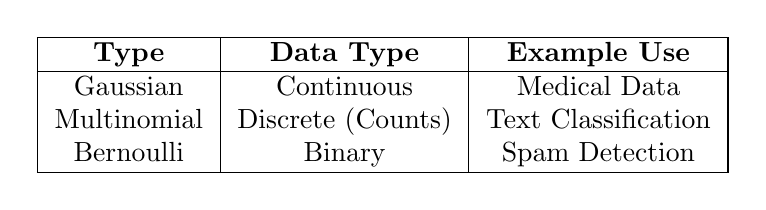
\begin{tikzpicture}
		\node at (0,0) {
			\begin{tabular}{|c|c|c|}
				\hline
				\textbf{Type} & \textbf{Data Type} & \textbf{Example Use} \\
				\hline
				Gaussian & Continuous & Medical Data \\
				Multinomial & Discrete (Counts) & Text Classification \\
				Bernoulli & Binary & Spam Detection \\
				\hline
			\end{tabular}
		};
	\end{tikzpicture}
\end{frame}

\Mysection{Python Implementation of Naive Bayes algorithm}

\begin{frame}{Steps to implement}
	\begin{figure}
		\centering
		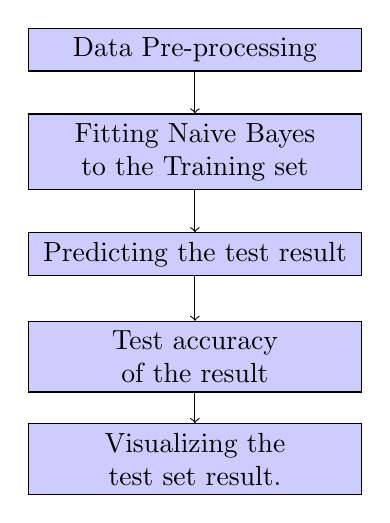
\begin{tikzpicture}[node distance=1.3cm, every node/.style={rectangle, draw, fill=blue!20, text width=4cm, align=center}]
			\node (input) {Data Pre-processing};
			\node (prob) [below of=input] {Fitting Naive Bayes to the Training set
			};
			\node (select) [below of=prob] {Predicting the test result
			};
			\node (output) [below of=select] {Test accuracy of the result
				
			};
			\node (visual) [below of=output] {Visualizing the test set result.
				
			};
			% Arrows
			\draw[->] (input) -- (prob);
			\draw[->] (prob) -- (select);
			\draw[->] (select) -- (output);
			\draw[->] (output) -- (visual);
		\end{tikzpicture}
		\caption{Naïve Bayes Classification Process}
		\label{fig:Naïve Bayes Classification Process}
	\end{figure}
\end{frame}

	\begin{python}
# Importing the libraries
import numpy as np
import matplotlib.pyplot as plt
import pandas as pd
# Importing the dataset
dataset = pd.read_csv('Social_Network_Ads.csv')
X = dataset.iloc[:, [2, 3]].values
y = dataset.iloc[:, -1].values
# Splitting the dataset into the Training set and Test set
from sklearn.model_selection import train_test_split
X_train, X_test, y_train, y_test = train_test_split(X, y, test_size = 0.25, random_state = 0)
# Feature Scaling
from sklearn.preprocessing import StandardScaler
sc = StandardScaler()
X_train = sc.fit_transform(X_train)
X_test = sc.transform(X_test)
# Training the Naive Bayes model on the Training set
from sklearn.naive_bayes import GaussianNB
classifier = GaussianNB()
classifier.fit(X_train, y_train)
# Predicting the Test set results
y_pred = classifier.predict(X_test)
# Making the Confusion Matrix
from sklearn.metrics import confusion_matrix
cm = confusion_matrix(y_test, y_pred)
print(cm)
# Visualising the Training set results optional
\end{python}

\Mysection{Pros and Cons}
	\begin{frame}{Pros and Cons of Naive Bayes Classifier}
	\begin{tikzpicture}[node distance=0.5cm]
		
		% Pros
		\node[draw, rectangle, fill=green!20, text width=3cm] (P1) at (0, 1) {Efficient};
		\node[draw, rectangle, fill=green!20, text width=3cm, below=of P1] (P2) {Simple to Implement};
		\node[draw, rectangle, fill=green!20, text width=3cm, below=of P2] (P3) {Good for Text Data};
		
		% Cons
		\node[draw, rectangle, fill=red!20, text width=3cm] (C1) at (5, 1) {Assumes Feature Independence};
		\node[draw, rectangle, fill=red!20, text width=3cm, below=of C1] (C2) {Zero-Frequency Problem};
		
		% Labels
		\node at (0, 2) {\textbf{Pros}};
		\node at (5, 2) {\textbf{Cons}};
		
	\end{tikzpicture}
\end{frame}





